% Journal of Aerosol Science manuscript (Elsevier elsarticle, author-year references).
% Check the current Guide for Authors before submission (highlights, graphical abstract, CRediT,
% data availability, declaration of generative AI use).
\documentclass[preprint,review,12pt,authoryear]{elsarticle}
\usepackage{amsmath,amssymb}
\usepackage{bm}
\usepackage{graphicx}
\usepackage{booktabs}
\usepackage{adjustbox}
\graphicspath{{figures/}}
\usepackage{siunitx}
\usepackage[hidelinks]{hyperref}
% Labels of the supplement, declared so that main.tex builds on its own (make_si_labels.py)
% Labels of the supplement, generated by make_si_labels.py from build/supplement.aux.
% Do not edit by hand; re-run the script when the numbering of the supplement changes.
\newlabel{S-sec:s-parts}{{S1}{1}{}{}{}}
\newlabel{S-tab:s_parts}{{S1}{1}{}{}{}}
\newlabel{S-sec:s-thermo}{{S2}{1}{}{}{}}
\newlabel{S-eq:s-first-law}{{1}{1}{}{}{}}
\newlabel{S-fig:s_residuals}{{S1}{1}{}{}{}}
\newlabel{S-tab:s_path}{{S2}{1}{}{}{}}
\newlabel{S-sec:s-qeff}{{S3}{1}{}{}{}}
\newlabel{S-fig:s_qext}{{S2}{1}{}{}{}}
\newlabel{S-sec:s-pform}{{S4}{1}{}{}{}}
\newlabel{S-eq:s-pumpspeed}{{5}{1}{}{}{}}
\newlabel{S-eq:s-massbalance}{{6}{1}{}{}{}}
\newlabel{S-eq:s-singleexp}{{8}{1}{}{}{}}
\newlabel{S-tab:s_pform}{{S3}{1}{}{}{}}
\newlabel{S-sec:s-pressure}{{S5}{1}{}{}{}}
\newlabel{S-fig:s_pressure}{{S3}{1}{}{}{}}
\newlabel{S-sec:s-npe}{{S6}{1}{}{}{}}
\newlabel{S-fig:s_heldout}{{S4}{1}{}{}{}}
\newlabel{S-sec:s-models}{{S7}{1}{}{}{}}
\newlabel{S-tab:s_models}{{S4}{1}{}{}{}}
\newlabel{S-sec:s-hvac}{{S8}{1}{}{}{}}
\newlabel{S-fig:s_humidity}{{S5}{1}{}{}{}}
\newlabel{S-fig:s_hvac}{{S6}{1}{}{}{}}
\newlabel{S-sec:s-nuisance}{{S9}{1}{}{}{}}
\newlabel{S-tab:s_nuisance}{{S5}{1}{}{}{}}
\newlabel{S-sec:s-cutoff}{{S10}{1}{}{}{}}
\newlabel{S-fig:s_cutoff}{{S7}{1}{}{}{}}
\newlabel{S-fig:s_envelope}{{S8}{1}{}{}{}}
\newlabel{S-sec:s-losses}{{S11}{1}{}{}{}}

% Line numbers start after the front matter: lineno and the first-page footnotes of elsarticle
% otherwise push the footnotes over the page footer.
\usepackage{lineno}

\journal{Journal of Aerosol Science}

\begin{document}

\begin{frontmatter}

\title{Working-fluid-free measurement of particle number concentration and water vapor from the
laser-extinction curve of an expansion cloud by simulation-based inference}

\author[tmu]{Nobuhiro Moteki\corref{cor1}}
\ead{moteki@tmu.ac.jp}
\cortext[cor1]{Corresponding author.}
\affiliation[tmu]{organization={Department of Chemistry, Graduate School of Science, Tokyo Metropolitan
                  University},
                  addressline={1-1 Minami-Osawa},
                  city={Hachioji},
                  state={Tokyo 192-0397},
                  country={Japan}}

\begin{abstract}
Condensation particle counters (CPCs) measure the total particle number concentration $N$ with a
working fluid such as butanol or water, which must be replenished and takes up water from humid
samples. We propose a working-fluid-free method that infers $N$ in real time with a homemade
apparatus of affordable general-purpose parts. In each 60-s cycle, sample air is expanded
in a flask, and the laser extinction by the cloud droplets that form on the particles
from the sample's own water vapor is recorded. The signal is interpreted by a physical model of the
expansion, the activation and growth of the droplets and the light reaching the photodiode, including
forward scattering. Neural posterior estimation inverts the model for $N$ and the water vapor mixing
ratio $q_w$. It averages over the unmeasured particle and instrument properties and needs no
calibration against a reference particle counter or hygrometer. In 52\,h of indoor measurements
(3114 cycles), the inferred $N$ agreed with a CPC (TSI 3022A) to a median ratio of 0.995
(interquartile range 0.950--1.046) with Pearson's $r = 0.997$ over 370--9500\,cm$^{-3}$. The 3-h
medians of this ratio ranged from 0.95 to 1.09. The inferred $q_w$ agreed with a chilled-mirror
hygrometer to a median ratio of 0.997. The largest uncertainties are the optical path and the
condensation coefficient. In theory, soluble particles activate down to dry diameters at or below
the 7-nm
50\,\% cutoff of the CPC. The method could enable monitoring of $N$ at many locations without a
working fluid.
\end{abstract}

\begin{keyword}
Particle number concentration \sep Condensation particle counter \sep Expansion cloud chamber \sep
Laser extinction \sep Simulation-based inference \sep Working-fluid-free
\end{keyword}

\end{frontmatter}
\linenumbers


\section{Introduction}
\label{sec:intro}
The number concentration of particles in air is dominated by ultrafine particles, 100\,nm or smaller
in diameter \citep{hei2013ultrafine,who2021global}. Because of their small size, they are inhaled
deeply into the lungs and can pass into the systemic circulation \citep{ohlwein2019health}. Their
health effects are under study \citep{ohlwein2019health}, and in urban areas their number
varies strongly in space and time \citep{kumar2014ultrafine}.
Yet they contribute little to the particle mass on which air-quality standards are based
\citep{hei2013ultrafine}.
The World Health Organization therefore recommends as good practice that the particle number
concentration above a lower size limit of 10\,nm or less be monitored alongside the regulated
pollutants \citep[Sect.~4.3]{who2021global}.
It characterizes 24-h means below 1000\,cm$^{-3}$ as low and 24-h means above 10\,000\,cm$^{-3}$
(or 1-h means above 20\,000\,cm$^{-3}$) as high.
Such monitoring needs many instruments that run
unattended for long periods.

The standard instrument for the total particle number concentration $N$ is the condensation particle
counter (CPC). In a CPC, particles grow by condensation of a supersaturated vapor to optically
countable droplets \citep{stolzenburg1991ultrafine}.
CPCs fall into two classes by the way the supersaturation is produced \citep{mcmurry2000history}.
In most continuous-flow CPCs, a steadily flowing sample is supersaturated by heat and vapor transfer in a
temperature-controlled growth tube \citep{agarwal1980continuous}. Expansion CPCs supersaturate a batch of
the sample by an adiabatic expansion and observe the droplets formed in each expansion cycle
\citep{miller1982supersaturation}.
Most CPCs in use today are of the continuous-flow type
\citep[p.~1476]{hering2025affordable}.
They count single droplets, and the
number concentration follows from the counts and the sample flow. Their counting efficiency near the
cutoff must be calibrated \citep{iso27891}. They need a working
fluid, usually butanol, isopropanol or water \citep{sem2002design,hering2005laminar}. Alcohols take up
water from humid samples: isopropanol does so within a few hours at 50\,\% relative humidity
\citep{sem2002design}, and the butanol of the TSI 3010 CPC should be drained and replaced weekly for the
same reason
\citep{tsi2002cpc3010}. Water vapor of a humid sample can also condense in the condenser and
contaminate the butanol, changing the lower counting limit. Some recent CPC models remove this water at
the cost of a
higher butanol consumption \citep{tsi2017cpc3750}.
Water-based CPCs that recover water from the sample air can run for weeks without
refilling under mild conditions, but they still rely on a wetted wick and on temperature-controlled
growth stages \citep{hering2019magic}. A recent affordable water-based particle counter of the expansion type
humidifies the sample through water-jacketed Nafion walls and optically counts the activated
droplets individually in each measurement cycle
\citep{hering2025affordable}.
Recently proposed affordable CPCs
\citep{yoo2019mems,collins2026opensource} also rely on a working fluid and on the precise
control of temperatures. Portable diffusion chargers avoid the working fluid but infer the number
from the charge acquired by the particles with an assumed dependence on their size
\citep{fierz2011design,asbach2024partector}.
\citet{gehin2004theoretical} proposed a continuous-flow particle counter in which the sample expands
in a nozzle and its own water vapor condenses on the particles. The proposal was a theoretical design.
To our knowledge, no experimental demonstration has been reported.

Expansion CPCs have the longer history and date back to the counter of \citet{aitken1889number}.
Using an expansion chamber, \citet{wilson1897condensation} found that drops also form in particle-free
air above a saturation ratio of about 4. Expansion CPCs must therefore keep the
maximum saturation ratio below this limit.
In the expansion particle counter of \citet{nolan1946calibration} the attenuation of a light beam by
the cloud was converted to a number concentration with a calibration table.
The table was built by successive dilution and anchored to direct droplet counts with Aitken counters
\citep{nolan1946calibration,pollak1959calibration}.
Automated versions that read the light scattered by the cloud remained in routine use for decades
\citep{skala1963new,mcmurry2000history}.

The calibration was needed because the extinction of the cloud depends not only on the number of
droplets but also on their size, and the size depends on the number because the droplets compete
for the available vapor \citep{wagner1975interdependence,wagner1975experimental}.
Later expansion CPCs avoided the calibration by reading the droplet size from Mie theory.
At the University of Vienna this principle was implemented as the constant-angle Mie scattering
method \citep{wagner1985cams}. The versatile size analyzing nuclei counter (vSANC) extends it to
several scattering angles \citep{pinterich2016vsanc}.
The extrema of the scattered light give the droplet size, and their height relative to the
transmitted light gives the number concentration without a reference particle counter.
The number concentration can also be obtained from this size and the extinction of the cloud
\citep{szymanski1990absolute}. The expansion-type Kelvin spectrometer uses the same principle
\citep{hollander2002theoretical}. It is an expansion CPC operated at controlled supersaturations.
An expansion CPC of the University of Mainz \citep{kurten2005automated} records over time the light
scattered at 1.1--4.4$^\circ$ by the growing droplets. The signal shows successive maxima and
minima as the droplets grow. Mie theory gives the droplet size at these extrema, and $N$
follows from the signal height there.
A later version with modified optics and a measured pressure drop \citep{saghafifar2009modified} no
longer needed an empirical calibration factor, but the times of the extrema had to be preselected
by an operator.
Its authors saw this as an obstacle to unattended operation and proposed fitting a model to the
whole intensity curve instead.
All these particle counters saturate the sample with the vapor of a working fluid (water or another
liquid) before the expansion.
They use purpose-built chambers and optics \citep{kurten2005automated,pinterich2016vsanc}.
Particle counters that use the absolute scattered intensity need the laser power calibrated before
each series of measurements \citep{kurten2005automated,saghafifar2009modified}.
In such chambers, measured growth curves of monodisperse particles at a controlled supersaturation
have also been inverted with a growth model to obtain the accommodation coefficients of water
\citep{winkler2004mass}.
Expansion CPCs that need no reference particle counter use only those prominent features of the light
intensity recorded during droplet growth at which Mie theory robustly determines the droplet size.
This keeps the inferred number concentration independent of the growth physics.
To our knowledge, the fit of the whole intensity curve proposed by \citet{saghafifar2009modified} has not
been realized,
possibly because the computational methods available at the time could not solve an inverse problem
that depends on the growth physics and on unmeasured properties of the particles and of the
instrument.

Here we show that the total particle number concentration $N$ can be measured quantitatively from the
laser-extinction curve of an expansion of sample air in a glass flask. No vapor is added to the sample.
The curve is recorded as the transmittance $\mathrm{Tr}(t)$ of the beam.
The method needs no working fluid, no calibration against a reference particle counter or
hygrometer and no optics beyond a laser and one photodiode.
Because nothing is added to the sample, the supersaturation reached depends on its unknown water
vapor mixing ratio $q_w$, which is therefore inferred together with $N$.
The first second of the extinction curve is used point by point instead of selected features.
It is interpreted by a physical model of the expansion and of the activation, growth and extinction of
the droplets, including the light that the droplets scatter into the photodiode.
The onset of the extinction carries $q_w$, and the spacing of the maxima of the extinction carries the
droplet size and hence $N$ (Sect.~\ref{sec:info}).
The inferred $N$ and $q_w$ depend on quantities that are not measured: the condensation coefficient,
the size distribution and hygroscopicity of the particles and imperfections of the recorded signal.
This dependence is handled by simulation-based inference \citep{cranmer2020frontier}.
It marginalizes these quantities over their plausible ranges, so that their uncertainty widens the
credible intervals instead of biasing the estimates, within the assumptions of the model. A 90\,\%
credible interval contains the true
value with 90\,\% probability, given the model and these ranges.
Neural networks have estimated posterior distributions in retrievals of the Earth's atmosphere
\citep{pfreundschuh2018neural}. Exoplanet atmospheres have been retrieved by neural posterior
estimation \citep{vasist2023neural}, the method used here.
The probability of a recorded curve given $q_w$ and $N$ (the likelihood) cannot be written down for
this forward model. Likelihood-free alternatives such as approximate Bayesian computation would need
many new simulations for every cycle. A trained neural network (the estimator) instead returns the posterior
distribution of $q_w$ and $N$ in a fraction of a second.
Each cycle is thus analyzed as soon as it is recorded, without any adjustment or intervention by an operator.
The transmittance is normalized to the intensity just before each expansion, so slow drifts of the
laser power and of the transmission of the flask wall cancel without any calibration.
All components except a photodiode amplifier and a relay board for the valves are affordable
general-purpose parts used without machining (Supplementary material, Sect.~\ref{S-sec:s-parts}).
The instrument evaluated here was built by the author. Third-year undergraduate students without
specialized engineering skills have built instruments of the same design in a laboratory course at
the University of Tokyo. They also built the circuits.
This paper demonstrates the inference and validates it against reference instruments in room air.
A laboratory characterization of the counter is left to a separate study (Sect.~\ref{sec:limitations}).

The paper is organized as follows. Section~\ref{sec:instrument} describes the instrument, the
reference instruments and the 52-h measurement of indoor air.
Section~\ref{sec:model} describes the forward model and Sect.~\ref{sec:inversion} the inversion.
Section~\ref{sec:evaluation} describes the evaluation design.
Section~\ref{sec:results} gives the results, and Sect.~\ref{sec:discussion} the uncertainty budget, a
comparison with earlier
expansion particle counters and the limitations.


\section{Instrument}
\label{sec:instrument}
\subsection{Chamber and flow system}
\label{sec:chamber}
The chamber is a round-bottom flask of borosilicate glass (HARIO MF-3L, nominal volume 3000\,mL; outer
diameter 202\,mm, wall thickness about 3\,mm, inner volume about 4\,L including the neck) closed by
a pre-drilled silicone stopper
(Fig.~\ref{fig:instrument}).
Two L-shaped stain\-less-steel tubes (1/4-in outer diameter, 0.035-in wall; inner diameter 4.6\,mm)
pass through
the stopper: the inlet ends about 10\,cm below the stopper (near the end of the neck) and the
outlet about 4\,cm below the stopper.
A third stainless tube (1/8-in outer diameter) through the stopper carries the thermistor cable
(the tube ends sealed with caulk), and a fourth port connects the pressure sensor.
Electrically conductive silicone tubing
(TSI 3001788, for 1/4-in fittings; inner diameter 0.19\,in, 4.8\,mm) connects the room-air inlet
through valve~1 to the flask (1.2\,m) and the flask
through valve~2 to the pump (1.9\,m). The valves are motorized ball
valves (KITZ ED24 series, DC 24\,V), which turn through 90$^\circ$ in about 5\,s and are switched by
a homemade relay board from the digital outputs of the data acquisition device.
The pump is an oil-free free-piston
pump (Nitto Kohki VP0940; 60\,L\,min$^{-1}$ free flow, ultimate vacuum $-533$\,hPa gauge, about
460\,hPa absolute), which runs
continuously. When valve~2 opens with valve~1 closed, the pressure in the flask falls from that of
the room (about 990\,hPa) to about 450\,hPa in 10\,s, close to the ultimate vacuum of the pump.
A similar flask and pump were used in our earlier work to study the thermodynamics of such expansions
\citep{moteki2013new} and the droplet size from coronae \citep{aoki2013corona}.

\begin{figure}[!htbp]
\centering
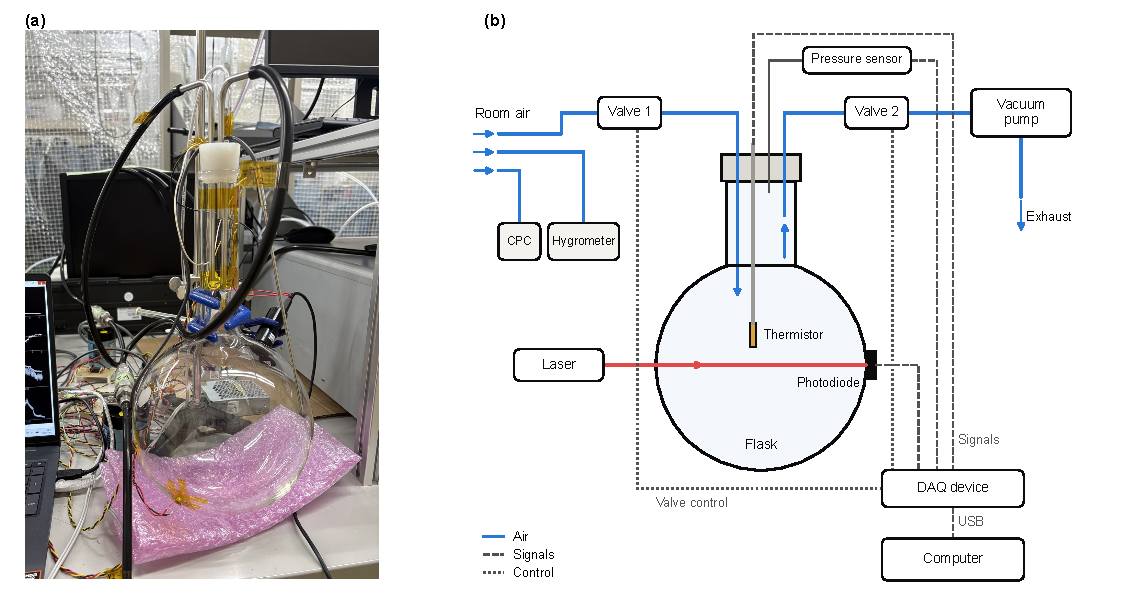
\includegraphics[width=\textwidth]{fig_instrument.pdf}
\caption{The instrument.
(a) Photograph.
(b) Schematic of the flow system, the optics and the sensors, and the reference instruments with
their own inlets.
Arrows show the air flow while both valves are open.}
\label{fig:instrument}
\end{figure}

\subsection{Sensors and data acquisition}
\label{sec:sensors}
A laser diode module ($\lambda = 670$\,nm, 3\,mW, beam diameter $\sim$1\,mm) sends its beam through
the center of the bulb to a Si photodiode (Hamamatsu S1223-01, active area 3.6\,mm $\times$
3.6\,mm) on the opposite side of the flask. Its TO-can package is fixed directly to the outer wall
with polyimide tape. The photocurrent is converted to a voltage (about +7\,V for the unattenuated
beam) by a homemade transimpedance amplifier.
A thin-film thermistor at the tip of the third tube gives the temperature of the air sealed in the
flask before the expansion.
The temperature follows from the thermistor resistance by the B-parameter equation ($B = 3435$\,K).
The resistance is measured with a voltage divider, and its value at 25\,$^\circ$C was calibrated at
one point against the thermocouple supplied with the hygrometer (accuracy $\pm0.1$\,K;
Sect.~\ref{sec:reference}).
The pressure in the flask is measured by a barometric pressure sensor (Setra 276, 0--1380\,hPa
absolute, i.e.\ 0--20\,psia, stated accuracy $\pm0.25$\,\% of full scale or $\pm3.4$\,hPa, time
constant 10\,ms; Sect.~\ref{S-sec:s-pform}), connected to the port in the stopper by
Tygon tubing (inner diameter 2\,mm, length 0.6\,m).
The pressure follows from the sensor output by its linear specification (0.1--5.1\,V for 0--1380\,hPa).
The three voltage signals are recorded at 100\,Hz by a 16-bit data acquisition device (NI USB-6210)
connected to a laptop computer, on which a Python program controls the valves, analyzes each cycle
and displays the results.

\subsection{Measurement cycle}
\label{sec:cycle}
The instrument repeats a cycle of 60\,s made of six phases of 10\,s.
(i) Flushing (valve~1 open, valve~2 open): the pump draws sample air through the flask.
(ii) Pressure equalization (valve~1 open, valve~2 closed): the flask returns to the room pressure
through the inlet.
(iii) Sealed (valve~1 closed, valve~2 closed): the median photodiode signal over this phase is the
reference intensity $I_0$, and $T_\mathrm{ini}$ and $p_\mathrm{ini}$ are the medians of the
temperature and pressure over its last second.
(iv) Expansion (valve~1 closed, valve~2 open): the pressure and the transmittance $\mathrm{Tr}(t)$
are recorded at 100\,Hz while the cloud forms and grows.
(v) Vent and (vi) wait (valve~1 open, valve~2 closed): the flask refills with sample air and the
cloud evaporates before the next flushing.
The data acquired in the expansion phase are analyzed (Sects.~\ref{sec:model}
and~\ref{sec:inversion}) as soon as it ends, and the inferred $q_w$ and $N$ are logged with the
recorded signals. 


\subsection{Pressure during the expansion}
\label{sec:pressure}
This section derives the analytic curve fitted to the measured pressure of each cycle, from which
the forward model computes the cooling and hence the supersaturation (Sect.~\ref{sec:model}).
The pump evacuates the flask toward an asymptotic pressure $p_\mathrm{off}$ (Pa), and the gas left in
the flask expands adiabatically.
For a well-mixed flask this gives an exponential approach of the pressure $p$ to $p_\mathrm{off}$ in
the time integral of $C(t)$, the effective pumping speed normalized by its value with the valve fully
open (derivation in Sect.~\ref{S-sec:s-pform}).
The pressure was first fitted with a single exponential and a valve that opens instantly at the
valve-opening onset $t_0$ (s).
This form leaves residuals of 4.0\,hPa rms (median over the cycles) in the first 2\,s after $t_0$,
when the cloud forms.
Two changes to this form were needed. First, the pumping speed grows while the ball valve opens. We take $C$
to grow linearly from 0 to 1 over the valve-opening duration $\Delta t_\mathrm{open}$ (s) and to stay
at 1 afterward.
Second, the decay deviates from a single exponential for reasons discussed in
Sect.~\ref{S-sec:s-pform}. We represent the deviation empirically by a second exponential:
\begin{equation}
\begin{aligned}
p(t) &= p_\mathrm{off} + (p_\mathrm{ini} - p_\mathrm{off})
\biggl[f_1 \exp\!\left(-\frac{1}{\tau_1}\int_{t_0}^{t} C(t')\,\mathrm{d}t'\right)\\
&\qquad + (1 - f_1) \exp\!\left(-\frac{1}{\tau_2}\int_{t_0}^{t} C(t')\,\mathrm{d}t'\right)\biggr],\\
C(t) &= \begin{cases}
0, & t < t_0,\\
(t - t_0)/\Delta t_\mathrm{open}, & t_0 \le t < t_0 + \Delta t_\mathrm{open},\\
1, & t \ge t_0 + \Delta t_\mathrm{open},
\end{cases}
\end{aligned}
\label{eq:pressure}
\end{equation}
where $\tau_1$ and $\tau_2$ (s) are the time constants of the fast and slow components and $f_1$
is the fraction of the fast component.
Both components are assumed to follow the same valve opening.
The linear opening makes the start of the drop quadratic and concave down for about 0.6\,s, a shape
that no sum of exponentials starting at $t_0$ can follow (Sect.~\ref{S-sec:s-pform}).
The valve opening alone reduces the early residual to 3.4\,hPa and the second exponential alone to 2.8\,hPa.
Both together in Eq.~(\ref{eq:pressure}) reduce it to 0.9\,hPa
(5--95\,\% of the cycles: 0.8--1.2\,hPa; Fig.~\ref{fig:pressure}).

Equation~(\ref{eq:pressure}) is fitted by least squares to the whole 10-s record of each expansion.
A 3-point running median first removes single-sample spikes from the valve motor.
$p_\mathrm{ini}$ is fixed at its measured value (Sect.~\ref{sec:cycle}). The other six parameters
are free: $t_0$, $\Delta t_\mathrm{open}$, $\tau_1$, $\tau_2$, $f_1$ and $p_\mathrm{off}$.
The onset $t_0$ must precede the first clear drop of the pressure. Its upper bound is therefore the
first time at which three consecutive samples lie more than 2\,hPa below $p_\mathrm{ini}$. Requiring
three samples ignores single noisy samples.
Within this bound $t_0$ is fitted from the whole quadratic start of the drop over about 0.6\,s rather
than from a single sample.
Hereafter, times are measured from $t_0$ ($t - t_0$ on the time axes of the figures).
The fitted $\Delta t_\mathrm{open}$ is only about 0.6\,s, although the ball valve takes about 5\,s to
turn through 90$^\circ$. This suggests that the flow area grows quickly at the start of the turn and
that the pump then limits the flow.
The fitted $p_\mathrm{off}$, $\tau_2$ and $f_1$ trade off against each other, but the fitted curves
are well determined (Sect.~\ref{S-sec:s-pressure}).
Our inference therefore uses the values of the fitted curves $p(t)$ at fixed times rather than their
parameters (Sect.~\ref{sec:obs}),
and the simulations draw recorded curves to cover their variation between cycles
(Sect.~\ref{sec:priors}).

\begin{figure}[!htbp]
\centering
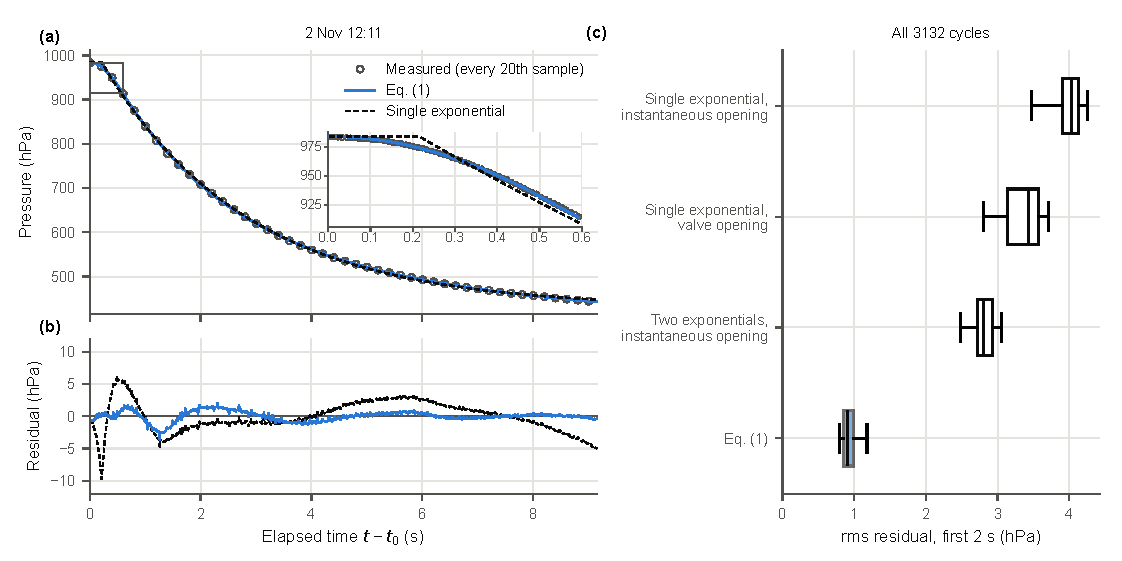
\includegraphics[width=\textwidth]{fig_pressure.pdf}
\caption{Pressure during the expansion. (a) Measured pressure of one cycle (3-point running median;
every 20th sample shown) with the fits of Eq.~(\ref{eq:pressure}) and of a single exponential with
instantaneous opening.
The inset shows all samples of the first 0.6\,s (box).
(b) Residuals of the two fits.
(c) rms residual over the first 2\,s after $t_0$ of the four forms of the
pressure curve for all cycles (box: interquartile range; whiskers: 5--95\,\%).}
\label{fig:pressure}
\end{figure}



\subsection{Measurement period and reference instruments}
\label{sec:reference}
The chamber was operated in a laboratory room of about 90\,m$^3$ from 31 Oct 12:18 to 2 Nov 16:49,
2026 (local time).
During this period the room air changed with the time of day, with the window open or closed and
with the air conditioning and an air purifier switched on or off.
The particle number concentration $N_\mathrm{CPC}$ measured by the CPC thus ranged over
370--9500\,cm$^{-3}$. The water vapor mixing ratio $q_{w,\mathrm{hyg}}$ from the hygrometer ranged over
5.8--9.2\,g\,kg$^{-1}$. Both instruments are described below.
The air was more
humid on 2 Nov than on the two other days.
A CPC (TSI 3022A) and a chilled-mirror
hygrometer (DPH-203B, Tokyo Opto-Electronics, Japan) sampled the room air through their own inlets,
5--10\,cm from the inlet of the chamber
and at the same height. $N_\mathrm{CPC}$ is taken as the 1\,Hz count divided by the sample
flow that the CPC reports each second (median 0.301\,L\,min$^{-1}$). A soap-film flow meter gave
0.298\,L\,min$^{-1}$. Two units of this
model agreed within 5\,\%. All values of $N_\mathrm{CPC}$ were below $10^4$\,cm$^{-3}$, where the
3022A counts single particles, with a live-time correction for coincidence above $10^3$\,cm$^{-3}$
\citep{sem2002design}.
For each cycle, $N_\mathrm{CPC}$ is the median over the 20\,s before
the expansion. The air sealed in the flask entered during the flushing 20--30\,s before the expansion,
which matters only for changes within a minute. The hygrometer (thermoelectrically cooled mirror, dew-point
range $-10$ to 20\,$^\circ$C, stated accuracy $\pm0.2$\,K) sampled continuously at 0.53\,L\,min$^{-1}$.
The reference mixing ratio $q_{w,\mathrm{hyg}}$ is computed from its dew point and $p_\mathrm{ini}$.


With the refill after the previous expansion and the flushing, an estimated 90\,\% of the air sealed
in the flask (about 4\,L) is replaced in each cycle, assuming that the flask is well mixed
(Sect.~\ref{S-sec:s-losses}). The chamber thus smooths the room air over little more than one cycle.
The comparability of the two particle counters in cutoff size and inlet losses is discussed in
Sect.~\ref{sec:comparability}.

\section{Forward model}
\label{sec:model}
The forward model computes the transmittance Tr$(t)$ of the laser beam from the
water vapor mixing ratio $q_w$ (kg\,kg$^{-1}$) and particle number concentration $N$ (kg$^{-1}$, number
per unit mass of dry air; see below) of the sample,
its temperature $T_\mathrm{ini}$ (K) and pressure $p_\mathrm{ini}$ (Pa) just before the expansion
(Sect.~\ref{sec:cycle}) and the fit of
Eq.~(\ref{eq:pressure}) to the recorded pressure $p(t)$.
The inversion uses only an inference window of about 1\,s at the start of the extinction
(Sect.~\ref{sec:obs}).
No air enters the flask during the expansion (valve~1 closed). The total water $q_w = q_v + q_l$
(vapor plus liquid, per unit mass of dry air; kg\,kg$^{-1}$) and the number of particles per unit mass
of dry air are therefore conserved. In the model $N$ is therefore this number (kg$^{-1}$). It is
converted to the number per volume (cm$^{-3}$) for reporting (Sect.~\ref{sec:npe}).

\subsection{Expansion thermodynamics}
\label{sec:thermo}
The temperature of the optically probed core of the flask follows from the first law for moist
air with condensation,
\begin{equation}
c_p \frac{dT}{dt} = -l_v \frac{dq_v}{dt} + T\,(R_d + q_v R_v)\,\frac{1}{p}\frac{dp}{dt},
\qquad c_p = c_{pd} + q_v c_{pv} + q_l c_l,
\label{eq:temperature}
\end{equation}
with the temperature $T$ (K), pressure $p$ (Pa) and time $t$ (s), the specific gas constants $R_d$
and $R_v$ of dry air and water vapor, the specific heats $c_p$ of the moist air and $c_{pd}$, $c_{pv}$
and $c_l$ of dry air, water vapor and liquid water (all J\,kg$^{-1}$\,K$^{-1}$), and the latent heat $l_v$
(J\,kg$^{-1}$). Without condensation, Eq.~(\ref{eq:temperature}) reduces to the dry adiabat. Expansion
counters use it to calculate their supersaturation from the pressure ratio
\citep{miller1982supersaturation}. Heat exchange with the wall is neglected (Sect.~\ref{sec:limitations}). The
saturation ratio
over a plane water surface is $S = e/e_s(T)$ with the vapor pressure $e = q_v
p/(\varepsilon +
q_v)$ (Pa), the saturation vapor pressure $e_s$ (Pa) and $\varepsilon = R_d/R_v$.
We express the supersaturation as $S - 1$ in percent.
The derivation and
the constants are given in Sect.~\ref{S-sec:s-thermo}.

\subsection{Activation and droplet growth}
\label{sec:growth}
The forward model assumes a model aerosol: a population of dry particles with a lognormal size
distribution (geometric mean radius $r_g$ (m;
count median diameter $2r_g$),
geometric standard deviation $\sigma_g$) and a uniform composition, with a single hygroscopicity
$\kappa$ at all sizes.
The distribution is divided into 12 bins that each contain one twelfth of the particles ($N/12$).
The bins are thus narrow near the median radius and wide in the tails of the distribution, rather than
equally spaced in log radius.
All particles of bin $j$ ($j = 1, \dots, 12$) are given the dry radius
$a_{d,j} = r_g \sigma_g^{z_j}$, where $z_j$ is the quantile of the standard normal distribution at
the cumulative fraction $(j - 1/2)/12$, that is, the center of the bin in number.
Each bin is followed in time as a moving bin, so that no remapping between size classes is needed,
and equal numbers place the computation where the particles are (convergence in
Sect.~\ref{S-sec:s-thermo}).
Each particle is a solution droplet of dry radius $a_d$ (m) and hygroscopicity $\kappa$
with the equilibrium saturation ratio \citep{petters2007single}
\begin{equation}
S_\mathrm{eq}(a) = \frac{a^3 - a_d^3}{a^3 - a_d^3(1-\kappa)}\,
\exp\!\left(\frac{2\sigma_w}{\rho_l R_v T a}\right),
\label{eq:koehler}
\end{equation}
where $a$ (m) is the droplet radius, $\sigma_w(T)$ (N\,m$^{-1}$) the surface tension and $\rho_l$
(kg\,m$^{-3}$) the density of water. At $t_0$ every particle is a haze droplet in equilibrium with the
initial saturation ratio.
The droplets grow by condensation
\citep[Eq.~13-28 with $S_\mathrm{eq}$ in place of $1 + y$]{pruppacher1997microphysics},
\begin{equation}
a\frac{da}{dt} = \frac{S - S_\mathrm{eq}(a)}{F_k + F_d},\qquad
F_k = \left(\frac{l_v}{R_v T} - 1\right)\frac{l_v \rho_l}{k_a' T},\qquad
F_d = \frac{\rho_l R_v T}{D_v' e_s(T)},
\label{eq:growth}
\end{equation}
where $F_k$ and $F_d$ (s\,m$^{-2}$) are the thermal and diffusional resistances. The diffusivity of
water vapor $D_v'$ (m$^2$\,s$^{-1}$) and the thermal conductivity of air $k_a'$
(W\,m$^{-1}$\,K$^{-1}$) are corrected for gas-kinetic effects \citep[Eqs.~13-14 and
13-20 with the vapor and thermal jump distances set to zero]{pruppacher1997microphysics},
\begin{equation}
D_v' = \frac{D_v}{1 + \dfrac{D_v}{\alpha_c a}\sqrt{\dfrac{2\pi}{R_v T}}},\qquad
k_a' = \frac{k_a}{1 + \dfrac{k_a}{\alpha_t a \rho_a c_{pd}}\sqrt{\dfrac{2\pi}{R_d T}}},
\label{eq:kinetic}
\end{equation}
where $\alpha_c$ is the condensation (mass accommodation) coefficient and $\alpha_t$ is the thermal
accommodation coefficient. $\alpha_t$ is set to 1 because expansion-chamber
measurements exclude values below 0.85 \citep{winkler2004mass}. With $\alpha_t = 0.85$, $N$ and
$q_w$ change by less than 0.5\,\%.
$\rho_a = p/(R_d T)$ (kg\,m$^{-3}$) is the density of the air, and $D_v(T, p)$ and $k_a(T)$ follow
\citet[Eqs.~13-3 and 13-18a]{pruppacher1997microphysics}.
The liquid water is $q_l = \tfrac{4}{3}\pi\rho_l \sum_j n_j a_j^3$ with $n_j = N/12$ (kg$^{-1}$)
droplets of radius $a_j$ (m) per unit mass of dry air in bin $j$.
Its growth removes vapor ($dq_v/dt = -dq_l/dt$) and so couples Eq.~(\ref{eq:growth}) to
Eq.~(\ref{eq:temperature}) and to $S$. Equation~(\ref{eq:temperature}) for $T$ and
Eq.~(\ref{eq:growth}) for the radii $a_j$ of the 12 bins, with $S_\mathrm{eq}$ from Eq.~(\ref{eq:koehler})
and $p(t)$ from Eq.~(\ref{eq:pressure}), thus form a system of 13 ordinary differential equations.
It is integrated in time from $t_0$ to the end of the simulation (4.2\,s) with an explicit Euler
scheme and a time step of 1\,ms. Within each step the radius of each bin is advanced in sub-steps
shorter than half its relaxation time. Haze droplets that relax faster than the time step are kept in
equilibrium with $S$ (Sect.~\ref{S-sec:s-thermo}). The same equations are used before
and after the droplets pass the critical radius, where $S_\mathrm{eq}(a)$ has its maximum. A bin
activates only if $S$ stays above this maximum long enough for its droplets to grow past the critical
radius. The activated fraction thus follows from the supersaturation reached during the expansion.

\subsection{Extinction including forward-scattered light}
\label{sec:forward}
The transmittance over the optical path $L$ (m) through the cloud is
\begin{equation}
\mathrm{Tr}(t) = \exp\!\left(-\pi L \rho_a \sum_j n_j a_j^2\, Q_\mathrm{eff}(a_j)\right),
\label{eq:tr}
\end{equation}
with $L = 0.18$\,m: the inner diameter of the flask less a cloud-free layer of about 1\,cm near the
wall on each side. The thickness of this
layer is an assumption based on experience with the chamber. Its uncertainty is assessed in
Sect.~\ref{sec:budget}.
The photodiode at the flask wall (Sect.~\ref{sec:sensors}) also receives the forward scattering
within the narrow cone it subtends, which is significant for droplets of a few micrometers.
We account for it as in the forward-scattering correction of extinction measurements
(\citealp{deepak1978forwardscattering1,deepak1978forwardscattering2};
\citealp[Sect.~4.4.3]{bohren1983absorption}),
which has also been applied in an expansion chamber \citep{szymanski1990absolute}.
The effective extinction efficiency is therefore
\begin{equation}
\begin{aligned}
Q_\mathrm{eff}(a) &= Q_\mathrm{ext}(a) - \left\langle \frac{1}{x^2}\int_0^{\theta_c(\ell)}
\left(|S_1(\theta)|^2 + |S_2(\theta)|^2\right)\sin\theta\,d\theta \right\rangle_\ell,\\
\theta_c(\ell) &= \arctan\frac{r_\mathrm{PD}}{\ell},
\end{aligned}
\label{eq:qeff}
\end{equation}
where $Q_\mathrm{ext}$ is the extinction efficiency, $x = 2\pi a/\lambda$ is the size parameter
with the wavelength $\lambda$ (m), $\theta$ (rad) is the scattering angle, $S_{1,2}$
are the Mie amplitude functions
\citep[Eq.~4.74]{bohren1983absorption}, $\theta_c$ is the half-angle of the cone that the photodiode subtends,
$r_\mathrm{PD} = 2.03$\,mm is the radius of the circle with the area of the photodiode, and
$\langle\cdot\rangle_\ell$ is the average over the distance $\ell$ (m)
between a droplet on the beam and the photodiode, taken uniformly over $\ell$ = 10--190\,mm.
The Mie quantities are computed for $\lambda = 670$\,nm and the refractive index
$1.33 + 2\times10^{-8}i$ and averaged over a small relative spread $s$ of the
droplet radius,
which smooths the fine ripples of $Q_\mathrm{ext}(a)$ and $Q_\mathrm{eff}(a)$.
The spread $s$ narrows as droplets grow by condensation, as $a^{-2}$ for radii much larger than the
kinetic length $(D_v/\alpha_c)\sqrt{2\pi/(R_v T)}$ in Eq.~(\ref{eq:kinetic}). The narrowing stops at a
prescribed lower bound of $s$, an ad hoc
allowance for broadening by processes
outside the model. Its value is drawn from a log-uniform prior distribution over 0.003--0.03
(Table~\ref{tab:priors}).
For a given droplet radius the correction is fixed by the area of the photodiode and its distance
from the beam ($r_\mathrm{PD}$ and $\ell$), so it has no adjustable parameter. It reduces the extinction by
3\,\% at $a = 1$\,\textmu m, 7\,\% at 2\,\textmu m and 11\,\% at 3\,\textmu m
(Sect.~\ref{S-sec:s-qeff}, Fig.~\ref{S-fig:s_qext}). Multiple scattering is neglected, as Tr stays
above 0.85 within the inference window.

\subsection{Information content of the extinction curve}
\label{sec:info}
\begin{figure}[!htbp]
\centering
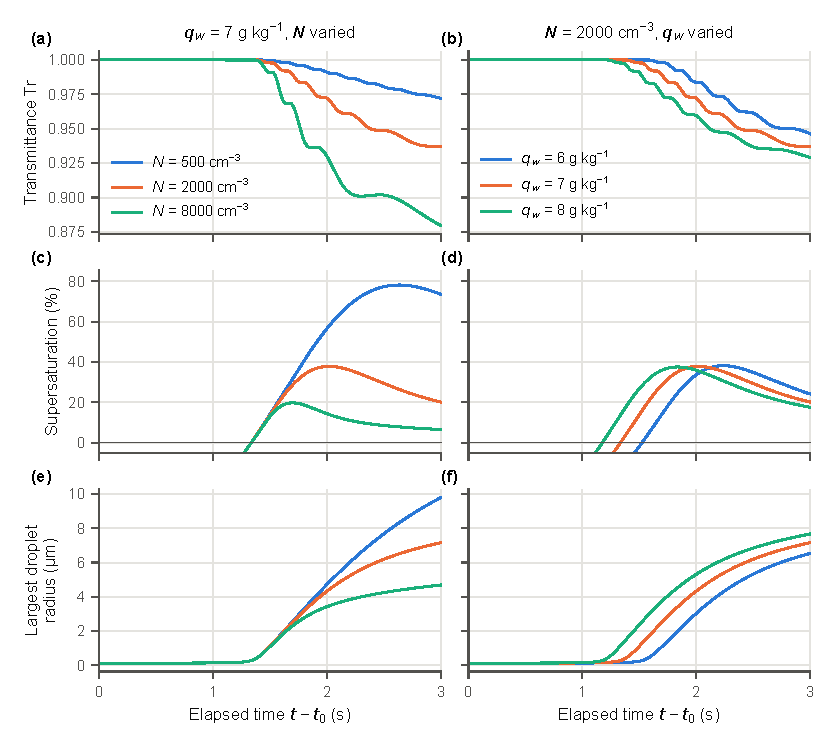
\includegraphics[width=\textwidth]{fig_sensitivity.pdf}
\caption{Forward model for the recorded pressure curve of Fig.~\ref{fig:pressure} ($T_\mathrm{ini} = 296$\,K,
$p_\mathrm{ini} = 984$\,hPa, reference values of the nuisance parameters in Table~\ref{tab:priors}): (a, b)
transmittance, (c, d)
supersaturation and (e, f) radius of the largest droplets, for (left) $N$ varied at
$q_w = 7$\,g\,kg$^{-1}$ and (right) $q_w$ varied at $N = 2000$\,cm$^{-3}$.}
\label{fig:sensitivity}
\end{figure}
Figure~\ref{fig:sensitivity} shows that $q_w$ and $N$ change different features of the Tr$(t)$ curve.
The onset of the extinction is sensitive to $q_w$ (right column). A higher $q_w$ brings the sample to
saturation earlier in the expansion, so the cloud appears earlier.
$N$ sets how many droplets share the condensing vapor (left column). At a given $q_w$, a higher
number concentration keeps the peak supersaturation lower (from 78\,\% at 500\,cm$^{-3}$ to 20\,\% at
8000\,cm$^{-3}$ in this example), and the droplets stay smaller. Although the droplets are smaller,
the extinction is larger because it scales with $N a^2 Q_\mathrm{eff}$.
As the droplets grow, the extinction passes through the broad maxima of $Q_\mathrm{eff}(a)$. The first
maximum of the extinction comes at the same time for all $N$ ($t - t_0 = 1.5$\,s, when the largest droplets
have grown to a
radius of about 1.1\,\textmu m; Fig.~\ref{fig:sensitivity}e). Later maxima are spaced more widely at high
$N$ because the
droplets grow more slowly (Fig.~\ref{fig:sensitivity}e). $N$ is thus encoded both in the depth of
the curve and, through the droplet size, in the spacing of the maxima. Expansion CPCs that need no
reference particle counter combine the extinction with the droplet size from Mie extrema in the same
way \citep{szymanski1990absolute,hollander2002theoretical}.

However, the effects of $q_w$ and $N$ on these features of Tr$(t)$ are entangled. $q_w$ also sets how
fast the droplets grow and hence the spacing of the maxima. The condensation coefficient and the
unmeasured properties of the particles shift both the onset and the spacing. Neither $q_w$ nor $N$ can
therefore be estimated from a single feature of the curve. Both have to be inferred from the shape of
the curve by inverting the forward model (Sect.~\ref{sec:inversion}).


\section{Inversion by simulation-based inference}
\label{sec:inversion}
The forward model has no closed-form likelihood: the observation depends on $q_w$ and $N$ through
the numerical solution of Eqs.~(\ref{eq:pressure})--(\ref{eq:qeff}) and on nuisance parameters
that are not measured (size distribution, hygroscopicity, condensation coefficient, droplet-size
spread and signal imperfections). We therefore use simulation-based
inference \citep{cranmer2020frontier}, of which \citet{deistler2025practical} give a practical
introduction.
The forward model is run many times with random values of all its inputs. Together with simulated
imperfections of the recorded signal (Sect.~\ref{sec:priors}) it forms the simulator.
From these runs a neural network learns to return the probability distribution (the posterior) of
$\bm{\psi} = (q_w, \log_{10}N)$ given an observation vector $\bm{y}$. We call this network the
estimator. The vector $\bm{y}$ collects the
measured Tr$(t)$ and $p(t)$ curves and the initial temperature $T_\mathrm{ini}$ of a cycle
(Sect.~\ref{sec:obs}).
The nuisance parameters are thereby averaged over their plausible ranges (the priors).

\subsection{Observation vector}
\label{sec:obs}
Each recorded cycle (Fig.~\ref{fig:cycle}) is reduced to the observation vector $\bm{y}$ of 115 numbers. The
transmittance is $\mathrm{Tr} = I/I_0$, with the photodiode signal $I$ and the reference intensity
$I_0$ of the sealed phase (Sect.~\ref{sec:cycle}). $t_\mathrm{s}$ is the onset of the extinction
(dashed lines in Fig.~\ref{fig:cycle}). It is the last time before Tr first reaches 0.985 at which Tr
still lies within the noise of its baseline before $t_0$ (Sect.~\ref{S-sec:s-npe}). In the simulations the
sample saturates ($S = 1$) 0.04--0.21\,s before
$t_\mathrm{s}$.
The vector contains $t_\mathrm{s}$ and Tr at 101 times from $t_\mathrm{s} - 0.10$\,s to
$t_\mathrm{s} + 0.90$\,s in steps of 10\,ms.
These times form the inference window.
It also contains $T_\mathrm{ini}$, $p_\mathrm{ini}$ and the pressure drop $p_\mathrm{ini} - p(t)$
of the fitted Eq.~(\ref{eq:pressure}) at 11 fixed times from 0.25 to 4\,s rather than the fit
parameters (Sect.~\ref{sec:pressure}).
We truncate the window at 0.9\,s after $t_\mathrm{s}$. At $N$ below 1000\,cm$^{-3}$ the measured Tr stops
falling about 1\,s after $t_\mathrm{s}$, while the simulated Tr continues to decrease
(Sect.~\ref{sec:limitations}).

\begin{figure}[!htbp]
\centering
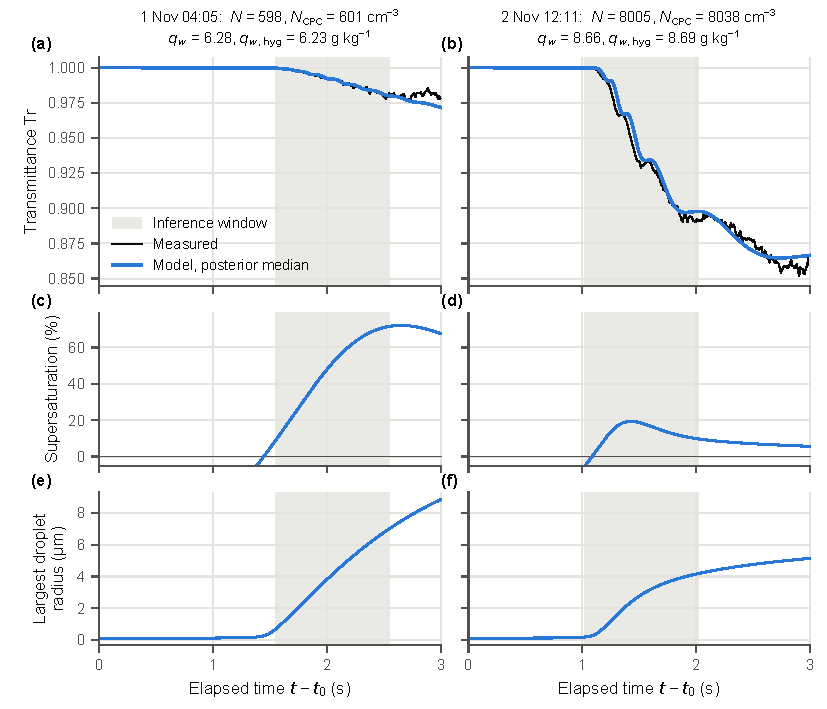
\includegraphics[width=\textwidth]{fig_cycle.pdf}
\caption{Two recorded cycles at low (left) and high (right) $N$. They are the cycles with $N_\mathrm{CPC}$
closest to 600 and 8000\,cm$^{-3}$ among those whose $N$ agrees with $N_\mathrm{CPC}$ within 2\,\%.
(a, b) Measured transmittance and the
forward model at the posterior median (leave-one-day-out estimate, reference values of the nuisance
parameters in Table~\ref{tab:priors}).
(c, d) Supersaturation and (e, f) radius of the largest droplets of the same simulation.
The shaded interval
is the inference window. Dashed lines: onset of the extinction $t_\mathrm{s}$ (Sect.~\ref{sec:obs});
dotted lines in (a, b): Tr = 0.985. The pressure of the right-hand cycle is shown in
Fig.~\ref{fig:pressure}.}
\label{fig:cycle}
\end{figure}

\subsection{Priors and nuisance parameters}
\label{sec:priors}

\begin{table}[!htbp]
\centering
\caption{Prior distributions of the simulator. $\mathcal{U}$: uniform distribution; log-$\mathcal{U}$:
log-uniform distribution; $\mathcal{N}(\mu, \sigma)$: normal distribution with mean $\mu$ and standard
deviation $\sigma$. The
spread $s$ is given at $a = 0.69$\,\textmu m, the first maximum of $Q_\mathrm{ext}$, and narrows with
growth. Reference values: used in calculations that run the forward model directly (e.g.,
Figs.~\ref{fig:sensitivity} and~\ref{fig:cycle} and Sects.~\ref{sec:sens} and~\ref{sec:comparability}).}
\label{tab:priors}
\begin{adjustbox}{max width=\textwidth}\small% Priors of the simulator (Python/cloudchamber/sbi_shape.py, sbi_shape4.py)
\begin{tabular}{llll}
\toprule
Group & Quantity & Prior & Note \\
\midrule
Inferred & Water vapor mixing ratio $q_w$ & $\mathcal{U}(3, 20)$\,g\,kg$^{-1}$ & \\
 & $\log_{10}N$ ($N$ in kg$^{-1}$) & $\mathcal{U}(8, 11)$ & $\approx$ 120--$1.2\times10^{5}$\,cm$^{-3}$ \\
\midrule
Chamber state & Initial temperature $T_\mathrm{ini}$ & $\mathcal{U}(288, 303)$\,K & in $\bm{y}$ \\
 & Initial pressure $p_\mathrm{ini}$ & $\mathcal{U}(980, 1030)$\,hPa & in $\bm{y}$ \\
 & Pressure curve & recorded curve & drop and time scaled by $\mathcal{U}(0.95, 1.05)$; \\
 & & of a training day & $\Delta t_\mathrm{open}$ shifted by $\mathcal{U}(-0.05, 0.05)$\,s \\
\midrule
Aerosol & Geometric mean dry radius $r_g$ & log-$\mathcal{U}(20, 80)$\,nm & lognormal, 12 bins; reference 40\,nm \\
 & Geometric standard deviation $\sigma_g$ & $\mathcal{U}(1.4, 2.2)$ & reference 1.8 \\
 & Hygroscopicity $\kappa$ & $\mathcal{U}(0.1, 0.7)$ & reference 0.3 \\
\midrule
Growth & Condensation coefficient $\alpha_c$ & log-$\mathcal{U}(0.1, 1)$ & reference 0.3 \\
 & Relative droplet-radius spread $s$ & log-$\mathcal{U}(0.015, 0.10)$ & at $a = 0.69$\,\textmu m; reference 0.04 \\
 & Lower bound of $s$ & log-$\mathcal{U}(0.003, 0.03)$ & reference 0.01 \\
\midrule
Signal & Width $\sigma_b$ of the smoothing of Tr & $\mathcal{U}(0, 0.05)$\,s & Eq.~(\ref{eq:smoothing}) \\
 & Error of the valve-opening onset $t_0$ & $\mathcal{N}(0, 0.01)$\,s & \\
 & Relative gain of Tr & $1 + \mathcal{N}(0, 3\times10^{-4})$ & \\
 & Noise standard deviation of Tr & log-$\mathcal{U}(10^{-4.5}, 10^{-3.5})$ & white, 100\,Hz \\
\bottomrule
\end{tabular}
\end{adjustbox}
\end{table}
Table~\ref{tab:priors} lists the priors. $q_w$ has a uniform distribution over 3--20\,g\,kg$^{-1}$.
$\log_{10}N$ has a uniform distribution over 8--11 with $N$ in kg$^{-1}$, which corresponds to about
120--$1.2\times10^5$\,cm$^{-3}$ in
the flask before the expansion. Both ranges are much wider than those of the room air. $T_\mathrm{ini}$
and $p_\mathrm{ini}$ have uniform distributions over 288--303\,K and 980--1030\,hPa. The pressure curve
of a simulation is that of a randomly chosen recorded cycle of the days used to train the estimator
(Sect.~\ref{sec:lodo}), with the pressure drop
and the time axis scaled by up to $\pm5$\,\% and the valve-opening duration $\Delta
t_\mathrm{open}$ shifted by up to
$\pm0.05$\,s, so that the simulations cover the pump and valve behavior actually encountered. The
aerosol and growth parameters span the values expected for indoor and urban air. Reported values of
the condensation coefficient $\alpha_c$ of water range from 0.03 to 1 \citep{mozurkewich1986aerosol}.
More recent experiments give values above 0.1 at atmospheric temperatures and close to 1 in
expansion chambers \citep{davidovits2004mass,winkler2004mass}.
The prior of $\alpha_c$ spans 0.1--1. The inference marginalizes $\alpha_c$ over this prior.
Unlike $\alpha_c$, the thermal accommodation coefficient is constrained well enough to be fixed
(Sect.~\ref{sec:growth}).

Calculations that run the forward model directly need one value for each
nuisance parameter (e.g., Figs.~\ref{fig:sensitivity} and~\ref{fig:cycle} and Sects.~\ref{sec:sens}
and~\ref{sec:comparability}). They use reference values (Table~\ref{tab:priors}). For a uniform prior
distribution
the reference value is the center of the range, which is also the median. For a log-uniform prior
distribution it is the
geometric mean of the two bounds, which is again the median. It is rounded to one significant digit. The
reference value of $\alpha_c$ is
thus 0.3
($\sqrt{0.1 \times 1} \approx 0.32$), lower than the value of 1 recommended for cloud
models \citep{laaksonen2005commentary}. The only exception is $\kappa$, set to 0.3 instead of the
center of its prior (0.4). This value lies within the range reported for continental aerosol
\citep{petters2007single}.

The simulated Tr is smoothed in time by a weighted moving average,
\begin{equation}
\widetilde{\mathrm{Tr}}(t) = \frac{\sum_k w_k\,\mathrm{Tr}(t - \tau_k)}{\sum_k w_k},\qquad
w_k = \exp\!\left(-\frac{\tau_k^2}{2\sigma_b^2}\right),
\label{eq:smoothing}
\end{equation}
where $\tau_k$ (s) are time differences in steps of 5\,ms up to $\pm4\sigma_b$. The width $\sigma_b$ (s) is
not known. For each simulation one value is drawn from a uniform distribution over 0--0.05\,s
(Table~\ref{tab:priors}) and used for the whole curve.
The smoothing allows for processes outside the model that would blur the curve, for example a cloud that
forms at slightly different times along the beam. The smoothed Tr is shifted in time by an error of the
valve-opening onset $t_0$, scaled by a small gain error and given white noise.
It is then resampled at 100\,Hz, and $t_\mathrm{s}$ and the samples of Tr are extracted from it by the
same procedure as for the recorded cycles (Sect.~\ref{sec:obs}).


\subsection{Neural posterior estimation}
\label{sec:npe}
The posterior is approximated by a conditional density $q_\phi(\bm{\psi} \mid \bm{y})$, a neural spline flow
\citep{durkan2019neural} whose parameters $\phi$ minimize
\begin{equation}
\mathcal{L}(\phi) = -\frac{1}{M}\sum_{i=1}^{M} \log q_\phi(\bm{\psi}_i \mid \bm{y}_i)
\label{eq:npe}
\end{equation}
over $M$ simulated pairs ($M \approx 20\,100$, 90\,\% of the 22\,304--22\,317 training pairs, with the rest
used to stop the training; Sect.~\ref{S-sec:s-npe}).
A neural spline flow maps a standard normal distribution onto a flexible distribution of $\bm{\psi}$
whose shape depends on $\bm{y}$, through a chain of invertible functions computed by a neural network.
A spline flow can represent skewed and curved posteriors, which arise from the entanglement of $q_w$
and $N$ (Sect.~\ref{sec:info}).
Since the pairs are drawn from the prior and the simulator, minimizing $\mathcal{L}$ makes
$q_\phi$ approach the true posterior for the curves that the simulator produces
\citep{papamakarios2016fast,greenberg2019automatic}.
The likelihood is never evaluated.
We use the \texttt{sbi} package \citep{tejerocantero2020sbi,boelts2025sbi} (version 0.27) with the
default settings of its neural spline flow.
Of 30\,000 simulations, about 81\,\% produce a cloud that reaches Tr = 0.985 within the simulated 4.2\,s.
The others are discarded (Sect.~\ref{S-sec:s-npe}), because $t_\mathrm{s}$ is not defined without a cloud.
The estimator thus excludes combinations of low $q_w$ and low $N$ that produce no measurable cloud.
Every recorded cycle produced a measurable cloud (Sect.~\ref{sec:results}).
Once trained, the estimator evaluates a new cycle without further simulations or training (it is
amortized). A recorded cycle is evaluated by drawing 1000 samples from
$q_\phi(\bm{\psi} \mid \bm{y})$, and we report the
median and the 5--95\,\% interval.
$N$ is converted from the number per unit mass of dry air to the number per volume at
$p_\mathrm{ini}$ and $T_\mathrm{ini}$.
On the laptop used for the measurements (AMD Ryzen 5 220, 16\,GB RAM, CPU only),
the complete processing of a cycle from the recorded signals to the posterior takes 0.08\,s
(median; 95th percentile 0.16\,s).
This is much shorter than the 60-s cycle.

\begin{figure}[!htbp]
\centering
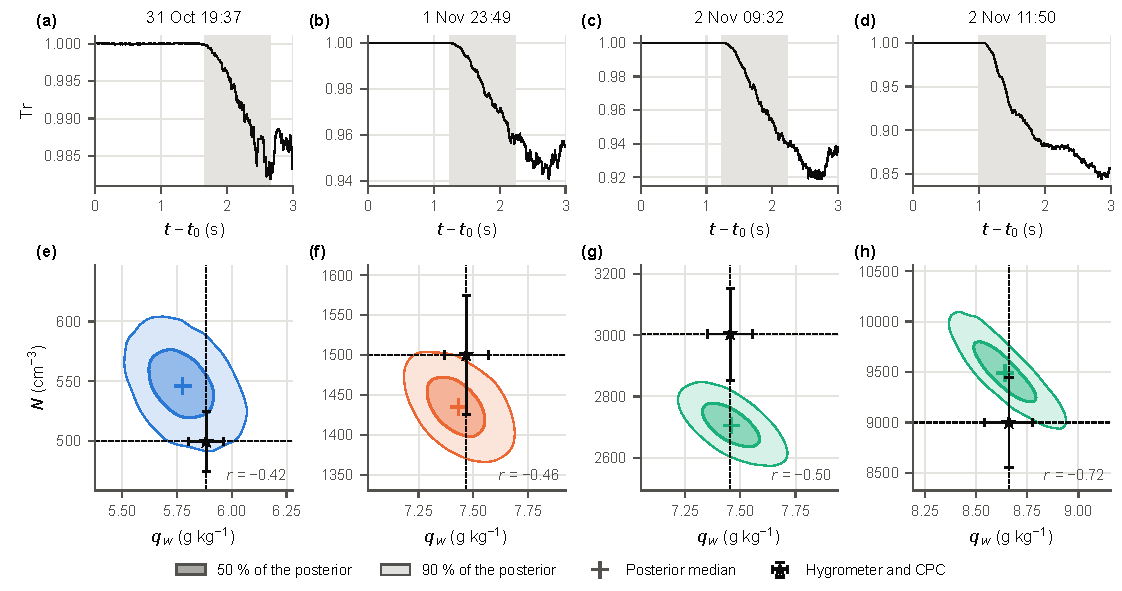
\includegraphics[width=\textwidth]{fig_posterior.pdf}
\caption{Joint posterior of $q_w$ and $N$ for four recorded cycles, chosen in advance by their day and
CPC value only (about 500, 1500, 3000 and 9000\,cm$^{-3}$; colors: 31 Oct blue, 1 Nov orange, 2 Nov
green). Each cycle is analyzed by the leave-one-day-out estimator
of its day (Sect.~\ref{sec:lodo}). (a, c, e, g) Measured transmittance with the inference window (shaded).
(b, d, f, h) Kernel density
estimate of 20\,000 samples of the neural spline flow, with the regions that contain 50\,\% and
90\,\% of the posterior and the posterior median. Stars and dashed lines: hygrometer and CPC values.
Error bars: their uncertainties ($\pm0.2$\,K in dew point and $\pm5$\,\%). $r$: Pearson's correlation
coefficient of $q_w$ and $\log N$ in the posterior samples.}
\label{fig:posterior}
\end{figure}

On 2000 simulations held out from the training, the rms error of the posterior median is
0.22\,g\,kg$^{-1}$ for $q_w$
and 5.9\,\% for $N$.
The 90\,\% credible intervals contain the true value in 91\,\% ($q_w$) and 90\,\% ($N$) of the cases
(Fig.~\ref{S-fig:s_heldout}).
This coverage test is recommended for checking simulation-based inference
\citep{talts2018validating,hermans2022trust}.

Figure~\ref{fig:posterior} shows the joint posterior of $q_w$ and $N$ for four recorded cycles over
the range of $N$. The cycles were chosen in advance by their day and CPC value only.
In all four the two quantities are negatively correlated, most strongly at high $N$. Pearson's
correlation coefficient $r$ between $q_w$ and $\log N$ in the posterior is $-0.42$ to $-0.72$.
A higher $q_w$ makes the droplets grow faster, so fewer of them reproduce the same extinction
(Sect.~\ref{sec:info}).
The 90\,\% credible intervals span about $\pm3$\,\% in $q_w$ and $\pm3$--8\,\% in $N$, widest at the
lowest $N$.


\section{Evaluation design}
\label{sec:evaluation}
\subsection{Data use and leave-one-day-out validation}
\label{sec:lodo}
Of the 3132 recorded cycles, 18 cycles during a separate aerosol-generation test near the inlets
(2 Nov 10:00--10:18) are excluded, and all other cycles are used. In the dense plumes of that test
the chamber and the CPC sampled different air (Sect.~\ref{S-sec:s-hvac}). The
validation is leave-one-day-out: each of the three days (31 Oct from 12:18, 1 Nov and 2 Nov) is
analyzed by an estimator trained without it. The recorded pressure curves drawn by its
simulator (Sect.~\ref{sec:priors}) come from the other two days.
The held-out day thus contributes nothing to the estimator that analyzes it.
The estimates use neither the CPC nor the hygrometer. The hygrometer value enters only the
sensitivity tests (Sect.~\ref{sec:sens}).

\subsection{Sensitivity tests}
\label{sec:sens}
To see what the forward-scattering correction contributes, an estimator was trained with a forward
model without it and evaluated on 2 Nov, the day held out from that estimator.
It is otherwise identical to the estimator trained on 31 Oct--1 Nov.
The nuisance parameters were tested with the forward model directly. $N$ and a time shift of up to
$\pm0.02$\,s were fitted to each of 104 recorded curves, with $q_w$ fixed at the hygrometer value, one
nuisance parameter at an edge of
its prior and the others at their reference values (Sect.~\ref{S-sec:s-nuisance}). The misfit combines the
difference in $t_\mathrm{s}$ and the rms difference
of Tr over the inference window. The optical path was varied in the same way
(Sect.~\ref{S-sec:s-thermo}).
Errors of the measured inputs were tested with the estimator itself. $T_\mathrm{ini}$ and
$p_\mathrm{ini}$ in $\bm{y}$ were shifted by their stated accuracies, and the pressure drops were
scaled by $\pm0.7$\,\%, the relative error of a drop of about 500\,hPa from an error of 3.4\,hPa.
The leave-one-day-out estimates were also compared with those of an estimator trained on all three
days (Sect.~\ref{S-sec:s-models}).


\section{Results}
\label{sec:results}
The chamber ran for 52\,h with two restarts (3 and 19\,min without data) and one slight realignment of
the laser. Every one of the 3132 recorded cycles produced an estimate within a second of the end of
the expansion (Sect.~\ref{sec:npe}). For the two cycles of Fig.~\ref{fig:cycle}, the simulation at the
posterior median reproduces the recorded transmittance within the inference window, with peak
supersaturations of 72\,\% and 19\,\%.

\subsection{Water vapor mixing ratio}
The inference accuracy of the mixing ratio $q_w$ is checked first. Because $q_w$ and $N$ are inferred
together, their errors are coupled: with $q_w$ fixed 3\,\% too low or too high, the fitted $N$ changes
by about 5--7\,\% in the opposite direction (Sect.~\ref{S-sec:s-nuisance}). An accurate $q_w$ is thus a
necessary condition for an accurate $N$.
Over the 3114 cycles (leave-one-day-out estimates; Fig.~\ref{fig:validation}a, c;
Table~\ref{tab:validation}), $q_w/q_{w,\mathrm{hyg}}$ has a median of 0.997 and an interquartile range (IQR)
of
0.987--1.007. The Pearson correlation coefficient of $q_w$ with $q_{w,\mathrm{hyg}}$ is $r = 0.992$. The
chamber also follows the hygrometer through the humid afternoon of
2 Nov (up to 9.2\,g\,kg$^{-1}$), above the range of the two other days. The hygrometer value lies
within the 90\,\% credible interval in 96\,\% of the cycles, so these intervals are slightly
conservative.

\begin{figure}[!htbp]
\centering
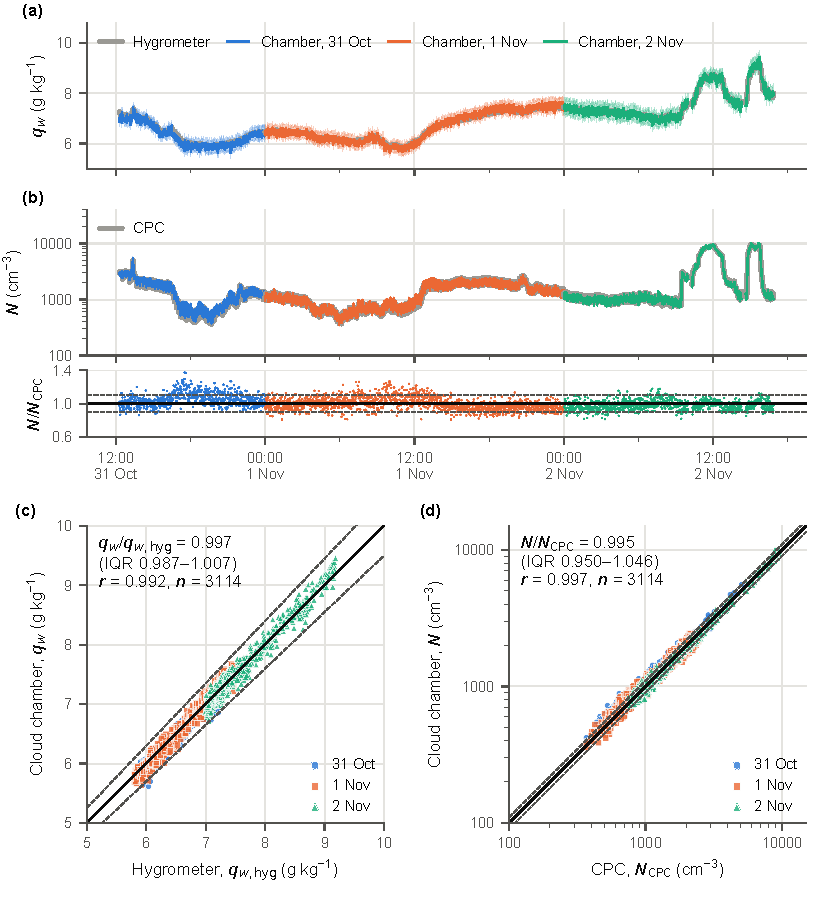
\includegraphics[width=\textwidth]{fig_validation.pdf}
\caption{Chamber against the references (leave-one-day-out estimates). (a) Water vapor mixing
ratio with the 90\,\% credible band and from the chilled-mirror hygrometer (Tokyo Opto-Electronics
DPH-203B). (b) Particle number concentration with the 90\,\% credible band and from the CPC
(TSI 3022A), and their ratio per cycle (dashed: $\pm10$\,\%). (c, d) Scatter plots of (a) and (b);
solid lines: 1:1, dashed: $\pm5$\,\% and $\pm10$\,\%. Colors: days of measurement.}
\label{fig:validation}
\end{figure}

\begin{table}[!htbp]
\centering
\caption{Leave-one-day-out validation: each day is analyzed by an estimator trained on the other two days.
Ranges of $q_{w,\mathrm{hyg}}$ and $N_\mathrm{CPC}$, median and interquartile
range (IQR) of the ratios, correlation of $N$ with $N_\mathrm{CPC}$, and the fraction of cycles
whose $q_{w,\mathrm{hyg}}$ or $N_\mathrm{CPC}$ lies in the 90\,\% credible interval (CI).}
\label{tab:validation}
\begin{adjustbox}{max width=\textwidth}\small% generated by Python/paper_table_validation.py
\begin{tabular}{lrlllllll}
\toprule
 & & & & \multicolumn{2}{l}{Water vapor mixing ratio} & \multicolumn{3}{l}{Particle number concentration} \\
\cmidrule(lr){5-6}\cmidrule(l){7-9}
Held-out day & Cycles & $q_{w,\mathrm{hyg}}$ & $N_\mathrm{CPC}$ & $q_w/q_{w,\mathrm{hyg}}$ & In 90\,\% CI & $N/N_\mathrm{CPC}$ & $r$ & In 90\,\% CI \\
 & & (g\,kg$^{-1}$) & (cm$^{-3}$) & median (IQR) & (\%) & median (IQR) & & (\%) \\
\midrule
31 Oct & 700 & 5.8--7.4 & 367--5050 & 0.989 (0.979--0.999) & 94 & 1.041 (0.995--1.099) & 0.993 & 47 \\
1 Nov & 1440 & 5.8--7.5 & 371--2656 & 1.000 (0.989--1.010) & 96 & 0.988 (0.943--1.043) & 0.988 & 41 \\
2 Nov & 974 & 7.0--9.2 & 746--9534 & 0.999 (0.989--1.008) & 98 & 0.981 (0.940--1.015) & 0.998 & 54 \\
\midrule
All & 3114 & 5.8--9.2 & 367--9534 & 0.997 (0.987--1.007) & 96 & 0.995 (0.950--1.046) & 0.997 & 46 \\
\bottomrule
\end{tabular}
\end{adjustbox}
\end{table}

\subsection{Particle number concentration}
\label{sec:resN}
The inferred $N$ follows the changes of $N_\mathrm{CPC}$ in the room air over more than an order of
magnitude, from 370\,cm$^{-3}$ in the evening and early morning to 9500\,cm$^{-3}$ with the window open,
including changes within minutes (Fig.~\ref{fig:validation}b, d). $N/N_\mathrm{CPC}$ has a median of 0.995
(IQR 0.950--1.046), $r = 0.997$ with $N_\mathrm{CPC}$, and the medians of the three days are 0.98--1.04
(Table~\ref{tab:validation}). The ratio varies over hours (Fig.~\ref{fig:validation}b). Its median over
consecutive 3-h intervals ranges from 0.95 to 1.09. It was highest (1.08--1.09) in the driest air of
31 Oct and 1 Nov. This air also had the lowest $N_\mathrm{CPC}$. On 2 Nov the median of each period was
0.95--0.97 with the air conditioning on and 1.00 with it off (Sect.~\ref{S-sec:s-hvac}).
The CPC value lies within the 90\,\% credible interval of $N$ in only 46\,\% of the cycles.
The variations and this low coverage are discussed in Sect.~\ref{sec:limitations}.

\section{Discussion}
\label{sec:discussion}
\subsection{Comparability with the CPC}
\label{sec:comparability}
The two instruments count particles above different sizes. The comparison is meaningful only if the
chamber activates at least the particles that the CPC counts, whose nominal 50\,\% cutoff diameter is
7\,nm \citep{sem2002design}. With the inferred $q_w$ and $N$ and the recorded pressure curves, the
forward model reaches peak supersaturations of 21--75\,\%, lower at higher $N$. By $\kappa$-Köhler
theory these activate soluble particles down to dry diameters of about 3--7\,nm ($\kappa$ = 0.1--0.3;
5--95\,\% of the cycles; Sect.~\ref{S-sec:s-cutoff}). Insoluble but wettable particles would need
4.5--12\,nm. In 19\,\% of the cycles, mainly at the lowest $N$, the peak comes after the inference
window, where the measured Tr departs from the model (Sect.~\ref{sec:obs}), so that the peak is less
certain there. Particles that the chamber counts but the CPC does not would make $N > N_\mathrm{CPC}$.

During the flushing the sample reaches the flask in turbulent flow. The CPC instead draws its
0.30\,L\,min$^{-1}$ through tubing of the same type in laminar flow. Diffusion losses are therefore
larger in the inlet of the CPC. For size distributions within the priors they raise $N/N_\mathrm{CPC}$
by about 1--5\,\% (Sect.~\ref{S-sec:s-losses}).

\subsection{Uncertainty budget and the role of the forward-scattering correction}
\label{sec:budget}
Table~\ref{tab:uncertainty} collects the contributions to the uncertainty of $N$ from the
sensitivity tests of Sect.~\ref{sec:sens}.

\begin{table}[!htbp]
\centering
\caption{Uncertainty budget of $N$ and of its comparison with the CPC, and the effect of removing the
forward-scattering correction. The estimator without it is trained like the full one and evaluated on
2 Nov. The relative error of the pressure drop corresponds to 3.4\,hPa in a drop of about 500\,hPa.}
\label{tab:uncertainty}
\begin{adjustbox}{max width=\textwidth}\small% generated by Python/paper_table_uncertainty.py
\begin{tabular}{lll}
\toprule
Element & Effect on $N$ & Basis \\
\midrule
\multicolumn{3}{l}{\textit{Forward-scattering correction (2 Nov, estimator trained on 31 Oct--1 Nov)}} \\
Full model & $N/N_\mathrm{CPC}$ = 0.981 ($q_w/q_{w,\mathrm{hyg}}$ = 0.999) & comparison on 2 Nov \\
Without the forward-scattering correction & $N/N_\mathrm{CPC}$ = 0.625 ($q_w/q_{w,\mathrm{hyg}}$ = 1.026) & comparison on 2 Nov \\
\multicolumn{3}{l}{\textit{Nuisance parameters at the edges of their priors}} \\
Condensation coefficient $\alpha_c$ (0.1, 1) & $+11.8$\,\%, $-2.8$\,\% & sensitivity fits (Sect.~\ref{S-sec:s-nuisance}) \\
Geometric mean dry radius $r_g$ (20, 80\,nm) & $-1.3$\,\%, $+2.1$\,\% & sensitivity fits (Sect.~\ref{S-sec:s-nuisance}) \\
Geometric standard deviation $\sigma_g$ (1.4, 2.2) & 0.0\,\%, 0.0\,\% & sensitivity fits (Sect.~\ref{S-sec:s-nuisance}) \\
Hygroscopicity $\kappa$ (0.1, 0.7) & $-0.7$\,\%, $+0.8$\,\% & sensitivity fits (Sect.~\ref{S-sec:s-nuisance}) \\
Droplet-radius spread (0.015, 0.10) & 0.0\,\%, 0.0\,\% & sensitivity fits (Sect.~\ref{S-sec:s-nuisance}) \\
Floor of the spread (0.003, 0.03) & 0.0\,\%, 0.0\,\% & sensitivity fits (Sect.~\ref{S-sec:s-nuisance}) \\
\multicolumn{3}{l}{\textit{Other}} \\
Days used to train the estimator & 0.8\,\% (IQR $-0.2$ to $+1.7$\,\%) & leave-one-day-out vs all-day estimator \\
Optical path $L = 0.18 \pm 0.01$\,m & $-6.8$\,\% (0.19\,m), $+7.7$\,\% (0.17\,m) & fits with the other path (Sect.~\ref{S-sec:s-thermo}) \\
Inlet losses, CPC vs chamber & $+0.7$ to $+5.1$\,\% in $N/N_\mathrm{CPC}$ & diffusion in the inlets (Sect.~\ref{sec:comparability}) \\
Initial temperature $T_\mathrm{ini}$ ($\pm0.1$\,K) & $\mp0.4$\,\% ($q_w$ $\pm0.7$\,\%) & estimator with shifted input \\
Initial pressure $p_\mathrm{ini}$ ($\pm3.4$\,hPa) & $\pm0.1$\,\% & estimator with shifted input \\
Pressure drop ($\pm0.7$\,\%, span and non-linearity) & $\pm0.1$\,\% ($q_w$ $\mp0.8$\,\%) & estimator with scaled input \\
Reference CPC & $\pm5$\,\% & two units compared \\
\midrule
Combined, without $\alpha_c$ and inlet losses & $\approx\pm9$\,\% & in quadrature \\
\bottomrule
\end{tabular}
\end{adjustbox}
\end{table}

The forward-scattering correction (Sect.~\ref{sec:forward}) is essential. With the plain
$Q_\mathrm{ext}$, $N/N_\mathrm{CPC}$ falls from 0.981 to 0.625 while $q_w$ is still retrieved
($q_w/q_{w,\mathrm{hyg}} = 1.026$).
The model then attributes the measured extinction to droplets that each extinguish more light and
so needs fewer of them.
The correction was added after an earlier version of the model without it had given $N$ far below
the CPC. However, the correction follows from the size and position of the photodiode alone and
contains no adjustable parameter. The agreement is thus not the result of a fit.

Among the nuisance parameters, the condensation coefficient has the largest effect
(Sect.~\ref{S-sec:s-nuisance}): $N$ is 12\,\% higher at $\alpha_c = 0.1$ and 3\,\% lower at
$\alpha_c = 1$ than at the reference value 0.3. Slower growth of each droplet must be compensated by
more droplets, and faster growth by fewer.
However, the fits at $\alpha_c = 0.1$ are worse (median misfit about five times that of the reference fits).
The curves thus disfavor $\alpha_c = 0.1$ but do not distinguish 0.3 from 1.
The other parameters change $N$ by at most 2.1\,\% (the geometric
mean dry radius has the largest effect among them). The spread of the droplet sizes has no effect
within the inference window,
consistent with the narrow droplet spectra in such chambers, which produce coronae
\citep{aoki2013corona,moteki2013new}. Per cycle, the leave-one-day-out estimate of $N$ is higher than that
of an estimator trained on all
three days by 0.8\,\% (median; IQR $-0.2$ to $+1.7$\,\%). Retrainings of one estimator with other
random seeds change $N$ by about as much (Sect.~\ref{S-sec:s-models}).

Among the fixed parameters of the model, the optical path is the least constrained.
With $L = 0.17$ or 0.19\,m instead of 0.18\,m, $N$ changes by $+8$ or $-7$\,\%.
The recorded curves fit worse with 0.19\,m than with 0.18\,m and slightly better with 0.17\,m
(Sect.~\ref{S-sec:s-thermo}).
An error of 0.1\,K in $T_\mathrm{ini}$ changes $N$ by 0.4\,\% and $q_w$ by 0.7\,\%. The stated accuracy
of the pressure sensor changes $N$ by about 0.1\,\% and $q_w$ by up to 0.8\,\%
(Table~\ref{tab:uncertainty}).
Without $\alpha_c$ and the inlet losses, the terms of Table~\ref{tab:uncertainty} combined in quadrature
amount to about $\pm9$\,\%, dominated
by the optical path (about $\pm7$\,\%) and the CPC ($\pm5$\,\%). A condensation coefficient as low
as 0.1 would add up to $+12$\,\%.
The observed median ratio of 0.995 is within these uncertainties.
The inlet losses alone would make the ratio 1--5\,\% higher (Sect.~\ref{sec:comparability}).
The curves slightly favor a path of 0.17\,m, which would raise the ratio by a further 8\,\%.
The path was kept at the value fixed beforehand from the geometry of the flask (Sect.~\ref{sec:forward}).


\subsection{Comparison with earlier expansion particle counters}
\label{sec:earlier}
The principles of the earlier expansion particle counters were described in Sect.~\ref{sec:intro}.
Their details also matter for the accuracy.
The vSANC reads the droplet size at five scattering angles with photomultipliers, lens--pinhole
optics and a reference detector \citep{pinterich2016vsanc}.
Even with a working fluid, the water vapor of the sample matters in that instrument.
Water and n-propanol nucleated together in particle-free air at high ambient humidity. This could
be neglected only because the events studied occurred at low humidity \citep{pinterich2016vsanc}.
Here the water vapor of the sample is the quantity that sets the supersaturation and is inferred.
The Mainz expansion CPC is the closest earlier approach because it also follows the signal of the
growing droplets in time. It linearizes the Beer--Lambert law and smooths the Mie ripples in the data. The
linearization
underestimates $N$ by 5\,\% at an optical thickness of 0.1.
When the depletion of the vapor suppresses the second pair of extrema, it has to fall back on the first
\citep{saghafifar2009modified}.
Here the exponential law and the variation of $\theta_c$ along the beam in Eq.~(\ref{eq:qeff}) are
included, and the Mie ripples are smoothed by the spread of droplet sizes in the model rather than
in the data.
Every cycle in 52\,h gave an estimate (Sect.~\ref{sec:results}).
The price of fitting the curve instead of reading selected features is that the estimate depends on
the growth model. Errors of the
growth model are covered only to the extent that the priors of its parameters contain the true values
(Sect.~\ref{sec:budget}).
Extinction is also a weaker signal than scattered light at low number concentrations because it is a small
change of a large baseline \citep{kurten2005automated}.
The consequence is stated in Sect.~\ref{sec:limitations}.

\subsection{Limitations}
\label{sec:limitations}
The slow variations of $N/N_\mathrm{CPC}$ (Sect.~\ref{sec:resN}) cannot be attributed to
humidity, particle number concentration, time of day or the state of the air conditioning, because these
changed together.
Because $q_w$ is retrieved without such variations, the cause most likely lies in the part of the
model that converts the curve into $N$.
Apart from the condensation coefficient, the nuisance parameters within their priors change $N$ by
at most 2.1\,\% (Sect.~\ref{sec:budget}).
The variations would thus require the condensation coefficient or the particles (size distribution
or composition beyond the priors) to change over time, or a process missing from the model.
Differences of this size between particle counters are common.
Expansion counters of the Nolan--Pollak type typically agreed within $\pm12$\,\% \citep{gras2002nolan}.
An expansion-type Kelvin spectrometer operated from first principles determines $N$ within about
$\pm15$\,\% \citep{hollander2002theoretical}.
The affordable expansion-type CPC of \citet{hering2025affordable} read about 15\,\% above the
benchtop CPCs it was compared with.

The variations are not represented in the model.
This is one reason why the credible intervals contain the CPC value in only 46\,\% of the cycles:
the intervals describe the uncertainty within the model, not the error of the model itself (processes
missing from it or parameters outside the priors). They also exclude the uncertainty of the CPC and
the terms of Table~\ref{tab:uncertainty} that are fixed in the simulator, such as the optical path.

The model also misses part of the extinction curve itself. After the inference window, the measured
Tr stops falling while the simulated Tr continues to decrease. At $N$ below 1000\,cm$^{-3}$ the
residual grows from about 1\,s after the onset of the extinction, $t_\mathrm{s}$. At higher $N$ it starts
later, at about 1.8\,s above 3000\,cm$^{-3}$ (Fig.~\ref{S-fig:s_residuals}). We therefore use the
recorded Tr only up to 0.9\,s after $t_\mathrm{s}$ (Sect.~\ref{sec:obs}).
The cause of this difference is not identified.
Conduction from the wall alone would warm the outer 1--2\,cm of the flask within the inference
window, which lies 1.1--2.6\,s after $t_0$ (5--95\,\% of the cycles; Sect.~\ref{S-sec:s-thermo}).
We also fitted the recorded curves with an optical path that shortens in time as this warm layer
grows. This path fits the window about as well as the constant path of 0.18\,m. After the window it
lowers the residual at high $N$ too much and leaves most of it at low $N$ (Table~\ref{S-tab:s_path}).
Such a layer therefore does not explain the difference.
Convection driven by small temperature differences is possible: in an expansion-type Kelvin
spectrometer, it limits the growth time more than conduction from the walls does
\citep{hollander2002theoretical}.

The evaluation covers 52\,h of indoor air in one room, with $N$ between 370 and
9500\,cm$^{-3}$ and $q_w$ between 5.8 and 9.2\,g\,kg$^{-1}$.
Lower $N$ gives shallower extinction curves (within the inference
window, Tr falls only to about 0.98 at 600\,cm$^{-3}$; Fig.~\ref{fig:cycle}a), so that $N$ is less
constrained (90\,\% credible interval about $\pm8$\,\% at 500\,cm$^{-3}$; Fig.~\ref{fig:posterior}).
Below about 90--160\,cm$^{-3}$ at $q_w$ = 6--9\,g\,kg$^{-1}$, and below 320--560\,cm$^{-3}$ at
3--4\,g\,kg$^{-1}$, the simulated cloud does not reach Tr = 0.985 and no estimate is made
($T_\mathrm{ini}$ = 23\,$^\circ$C; Fig.~\ref{S-fig:s_envelope}).
Higher $N$ and outdoor air have not been tested.
The recorded $p_\mathrm{ini}$ (982--993\,hPa) lay near the lower edge of its prior (980\,hPa).
Measurements over a wider range of $p_\mathrm{ini}$, as at higher altitude or in other weather, are
needed to train and test the estimator there.
The priors assume a single lognormal mode with a count median
diameter of 40--160\,nm, so that air dominated by freshly nucleated particles is outside them.
In dry air the expansion must go further before the sample saturates.
The supersaturation reached and hence the cutoff size then depend on the humidity of the sample,
which matters most in cold or dry seasons (Fig.~\ref{S-fig:s_envelope}). In warm, dry air
(2\,g\,kg$^{-1}$ at 30\,$^\circ$C) no measurable cloud forms. In cold air with few particles the
peak saturation ratio can exceed 4, where drops also form without particles. Operation outside the
priors ($q_w$ = 3--20\,g\,kg$^{-1}$, $T_\mathrm{ini}$ = 288--303\,K) requires retraining the
estimator.
The cutoff itself is known only from theory (Sect.~\ref{sec:comparability}).

A laboratory characterization is the next step. It should measure the counting efficiency against
particle size with classified particles and an electrometer, and the zero and the detection limit
with filtered air. It should also test the estimator, kept unchanged, in another period, in outdoor
air and in dry and cold seasons, together with measured size distributions.

\section{Conclusions}
Monitoring of the particle number concentration is recommended alongside the regulated pollutants.
It needs many instruments that run unattended for long periods. Condensation particle counters need a
working fluid. Earlier expansion particle counters saturated the sample with one, and some relied on a
reference particle counter or on settings made by an operator.
We have shown that an expansion chamber made of a glass flask, two motorized valves, a pump, a
laser, one photodiode, a pressure sensor and a thermistor measures $N$ with none of these.
The only condensing vapor is the water vapor of the sample, and no reference instrument is needed
apart from a one-point calibration of the thermistor.
It is built from affordable general-purpose parts without machining, and undergraduate students
have built instruments of the same design in a laboratory course.

The key is to interpret the shape of the extinction curve of the cloud with a physical model of its
formation and growth. Neural posterior estimation inverts this model. It infers the water vapor of the
sample together with $N$ and takes the place of both the reference particle counter and the operator.
The chamber ran for 52\,h with two restarts and one slight realignment of the laser.
Over 370--9500\,cm$^{-3}$, $N$ agreed with a CPC to a median ratio of 0.995 ($r = 0.997$), within
the uncertainty of the comparison (about $\pm9$\,\%, excluding the condensation coefficient and the
inlet losses).
The inferred $q_w$ agreed with a chilled-mirror hygrometer to a median ratio of 0.997.
In theory, the chamber activates soluble particles at least as small as those counted by the CPC.
Variations of the 3-h median ratio between 0.95 and 1.09 remain unexplained.
A working-fluid-free particle counter that is simple to build
thus appears feasible for unattended monitoring of the particle number concentration, once characterized in
the laboratory and tested in outdoor air and over wider ranges of pressure and humidity.

\section*{CRediT authorship contribution statement}
\textbf{Nobuhiro Moteki:} Conceptualization, Methodology, Software, Validation, Formal analysis,
Investigation, Resources, Data curation, Writing -- original draft, Writing -- review \& editing,
Visualization, Project administration, Funding acquisition.

\section*{Declaration of generative AI and AI-assisted technologies in the manuscript preparation process}
During the preparation of this work the author used Claude (Anthropic) in order to draft and edit the
text, write analysis and plotting code, and check the references. After using this tool, the author
reviewed and edited the content as needed and takes full responsibility for the content of the
published article.

\section*{Funding}
This work was supported by JSPS KAKENHI [grant numbers 23K28210,
23K28221, 23H00524], the Environmental Research and Technology
Development Fund (JPMEERF20232001, JPMEERF20262002) of the Environmental Restoration
and Conservation Agency of Japan, and the TMU Selected Research
Support for Young Researchers (Promising Research).

\section*{Declaration of competing interest}
The author declares no known competing financial interests or personal relationships that could have
appeared to influence the work reported in this paper.

\section*{Data availability}
{\sloppy The code for the instrument control, the forward model, the inference and the figures of this paper
is available at \url{https://github.com/NobuhiroMoteki/CloudChamberExperiment}. The recorded data
(pressure and transmittance of every cycle, the estimates, and the CPC and hygrometer records) are
archived at Zenodo \citep{moteki2026data}, \url{https://doi.org/10.5281/zenodo.24070205}.\par}

\section*{Acknowledgements}
The author thanks Dr. N. Takegawa (Tokyo Metropolitan University) for the use of a second CPC
(TSI 3022A) and for useful comments.
This work was inspired by the author's teaching of the undergraduate laboratory course at the
University of Tokyo in which students built instruments of the same design.

\bibliographystyle{elsarticle-harv}
\bibliography{refs}

\end{document}
